\section{Program Description}
In this section we will be going over how the program as a whole will function using flowcharts to illustrate the flow of the program. In the below figure (\ref{fig:Main_Flowchart}) the overall flow of the program can be seen. As we mentioned in the requirements section the program will be accepting a \verb|.csv| file. This input file first has to be read and parsed in order to convert the file into a data structure that we can use within our program. Once the input file has been processed we need to determine if any changes are necessary. This is done by comparing the expected work time (from the input file) with the work time that has been scheduled so far.

\begin{figure}[ht!]
    \centering
    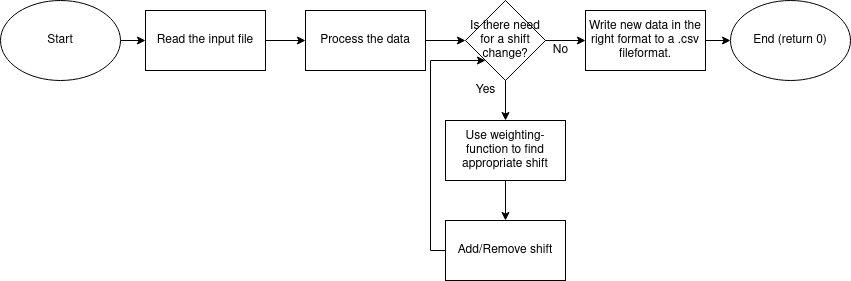
\includegraphics[width=\textwidth]{media/Flowcharts/General Flowchart.png}
    \caption{Flowchart of the program flow.}
    \label{fig:Main_Flowchart}
\end{figure}

If there is either too much or too little work time scheduled the program will remove or add scheduled time, respectively. In order to determine where to add or remove a time slot a weighting function will be used. Once a time slot has been removed or added the program will once again check the total time and compare it to the expected amount. If they match, the program will proceed. Otherwise, the aforementioned process will repeat. Once this process has finished the resulting schedule will be formatted and written to a file.

As mentioned the weighting function will be used to determine which time slot should be added or removed. It does this by giving each time slot a score, here the highest score will be the time slot which will be removed and the lowest score will be added. A flowchart of this function can be seen on Figure \ref{fig:weighting_flow}.

\clearpage
\begin{figure}[ht!]
    \centering
    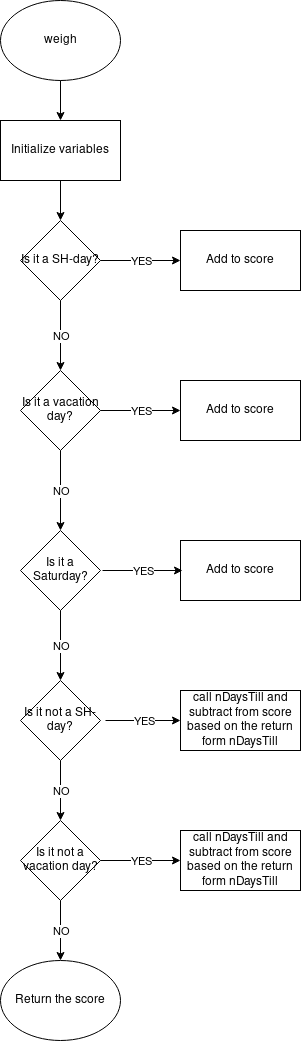
\includegraphics[width=0.4\textwidth]{media/Flowcharts/weight_flow.png}
    \caption{Weighting function flowchart.}
    \label{fig:weighting_flow}
\end{figure}

The most important part of the function is the five if-statements and the code being run if these turn out to be true. In the first three we check for whether or not it is a specific day. If it is we add to the score. This means that time slots in these days they will get a better score. Then we check for whether or not it is an sh-day or vacation day in the last two if-statements. If it is not an sh-day we calculate the number of days too the closest sh-day. We then multiply the number of days with a constant and subtract that from the score. The same process is done for vacation days. 

To calculate the aforementioned number of days we use the nDaysTill function. A flowchart for that con be seen on Figure \ref{fig:flow_nDaysTill}.

\clearpage
\begin{figure}[ht!]
    \centering
    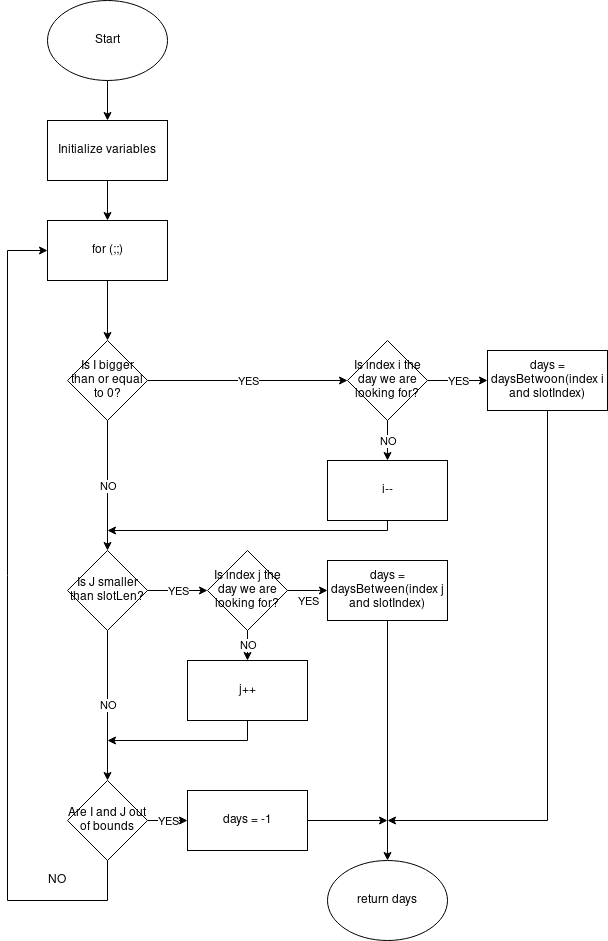
\includegraphics[width=\textwidth]{media/Flowcharts/nDaysTill_flow.png}
    \caption{Flowchart for the nDaysTill function.}
    \label{fig:flow_nDaysTill}
\end{figure}

This function starts off by making two index variables (i and j) based on an index it gets as a parameter. The first is going to go backwards in a time slot array and the other is going to go forwards in the same array. We then go into an infinite loop. In the loop there are three if statements, the first checks whether i is out of the array bounds, the second does the same but for j and the last checks both the variables. If the first if statement is true we then check to see if the time slot at index i is on the day that we are looking for, if it is we calculate the number of days between the time slot at the index given as a parameter and the time slot at index i. We then break out of the loop and return the number of days. If it turns out that it is not the day we are looking for we subtract one from i and go back to the for loop right after the first if statement. The second if statement has the same process as the first except this time we check j. Lastly we check to see if both index variables are out of the array bounds, and if they are we break out of the loop and return -1.